\section{Metodología del Proyecto}
En esta sección, se describirá la metodología para abordar tanto el
desarrollo del software como la propia metodología de investigación. La metodología
de desarrollo de software se basa en el uso de metodologías ágiles\cite{Agile_Microsoft}, concretamente
en la metodología Scrum\cite{Atlassian_Scrum}. Por otro lado, la metodología de investigación es una
metodología propia diseñada para abordar problemas dentro del marco de trabajo de
los problemas combinatorios NP-Hard diseñada por el autor de este trabajo. Esta
metodología se basa en el uso de técnicas de IL.

\subsection{Metodologías ágiles}
Las metodologías ágiles son un conjunto de metodologías de desarrollo de software
que se caracterizan por ser iterativas e incrementales. Estas metodologías se
basan en el desarrollo de software en ciclos cortos de tiempo, llamados
iteraciones, en los que se desarrolla una parte del software. Estas iteraciones
son incrementales, es decir, cada iteración añade una funcionalidad al software
que se está desarrollando. De esta forma, se consigue que el software se
desarrolle de forma incremental, y que se pueda ir probando y testeando a medida
que se desarrolla. Esto permite que se puedan detectar errores de forma temprana
y que se puedan corregir de forma rápida. Además, permite que el software se
pueda adaptar a los cambios que se produzcan en los requisitos del proyecto.\medskip

A diferencia de las metodologías tradicionales o pesadas\cite*{Jose_1634898355000} 
(como por ejemplo el modelo en cascada), las metodologías ágiles no se basan en la planificación
inicial del proyecto, sino que se basan en la adaptación constante, cualidad
que es muy importante especialmente en proyectos de investigación, en los que
la planificación inicial es muy difícil de realizar debido a la incertidumbre
que existe en este tipo de proyectos y a los diversos factores externos que
pueden afectar al proyecto.

\begin{figure}[ht]
    \centering
    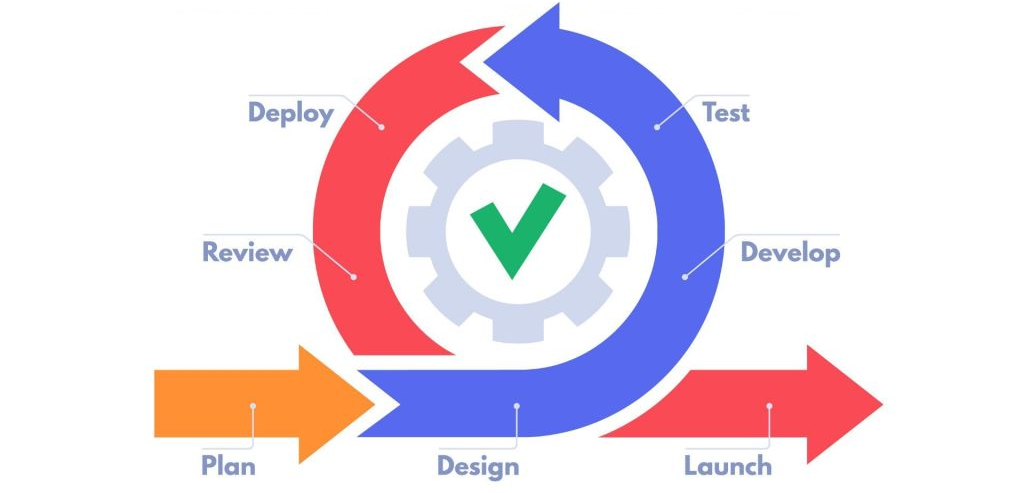
\includegraphics[width=\textwidth]{agile.png}
    \caption{Flujo de trabajo de una metodología ágil.}
    \label{fig:agile}
\end{figure}

\subsection{Metodología de desarrollo}
MLOps (Machine Learning Operations) es una extensión de la metodología DevOps (Development Operations)
que se enfoca en la integración, desarrollo y gestión del software de la mano del ciclo de vida del modelo.
Los pilares fundamentales se basan en la automatización y la mejora progresiva de la calidad del modelo,
lo que permite una implementación y puesta en producción mucho más efectiva. Para lograrlo, utiliza herramientas
y técnicas que permiten monitorizar, testear, mejorar y adaptar no solo los modelos sino toda la arquitectura
del sistema de forma continua y escalable. Aquí podemos observar el flujo de información dentro de una
arquitectura MLOps.

\begin{figure}[ht]
    \centering
    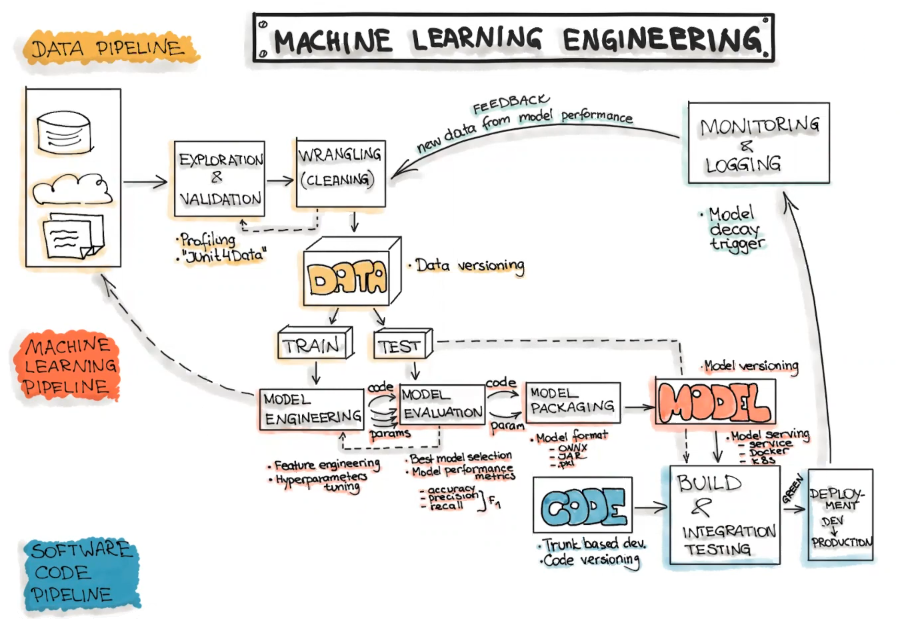
\includegraphics[scale=0.55]{architecture.png}
    \caption{Arquitectura MLOps}
    \label{fig:architecure-mlops}
\end{figure}

\subsubsection{Principios de MLOps}
A continuación, vamos a detallar los principios de MLOps que vamos a seguir en el desarrollo de nuestro proyecto.
En esta sección se incluyen los puntos más importantes de la metodología, durante todo el desarrollo intentaremos
cumplir con ellos en la medida de lo posible, ya que pueden darse situaciones en las que sea totalmente imposible
satisfacerlos al completo.

\begin{itemize}
    \item \textbf{Automatización}: la automatización es la clave para la eficiencia y la escalabilidad.
          Aqui incluimos tareas como la generación de datos, el despliegue del modelo, la evaluación y
          la puesta en producción.
    \item \textbf{Testeo}: garantiza que tanto la funcionalidad como el desempeño del modelo están evaluados correctamente.
          Esencial en Machine Learning para identificar problemas y mejorar la confianza en los resultados.
    \item \textbf{Versionado}: es importante tener un control de versiones de los datos, el código y los modelos.
          Puede variar el método dependiendo de la herramienta que se utilice, pero existen estándares como Git para la gestión
          de código y GitHub/GitLab para el almacenamiento de los repositorios.
    \item \textbf{Reproducibilidad}: es necesario poder reproducir los resultados de forma consistente, puede ser
          complicado en Machine Learning debido a la naturaleza aleatoria de los algoritmos. Igualmente aquí se trataran
          las herramientas y medidas necesarias para lograrlo.
    \item \textbf{Monitorización}: es importante tener un control de los modelos en proceso de entrenamiento o de producción.
          Por ello, recolectar estadisiticas en tiempo de procesamiento nos ayudará a generar nuevas hipotesis para las proximas interaciones.
\end{itemize}

\subsubsection{Flujo de trabajo}
Una de las características de los proyectos de Machine Learning es que son tecnologías en constante evolución, el
desarrollo no es un proceso sencillo y requiere de un enfoque coordinado por parte de los diferentes
equipos que lo conforman para asegurar su sostenibilidad a largo plazo. Es fundamental poder adapatarse a los cambios
de forma agil, sin que esto suponga un deterioro del nivel de productividad o que ralentice el avance de nuevas
funcionalidades.\medskip

Podemos identificar tres fases principales: diseño, desarrollo del modelo y operaciones. Cada fase tiene un enfoque
específico y requiere una serie de tareas para garantizar el éxito del proyecto. La fase de diseño,
se definen los objetivos y requisitos del proyecto, se identifican los datos necesarios para el entrenamiento y
se establecen los criterios de éxito. La fase de desarrollo del modelo, se preparan los datos, se entrena el modelo
y se evalúa su rendimiento. También se realiza la validación y se toman las decisiones sobre el modelo final a utilizar.
Finalmente, en la fase de operaciones, se integra el modelo en la infraestructura existente, se monitorea su rendimiento
y se extraen conclusiones para futuras iteraciones. Al repartir las responsabilidades en diferentes fases, aislamos los erroes junto con la carga de trabajo y podemos avanzar
sin la preocuapacion de que un bug o un cambio requisitos afecte al resto del equipo.

\begin{figure}[ht]
    \centering
    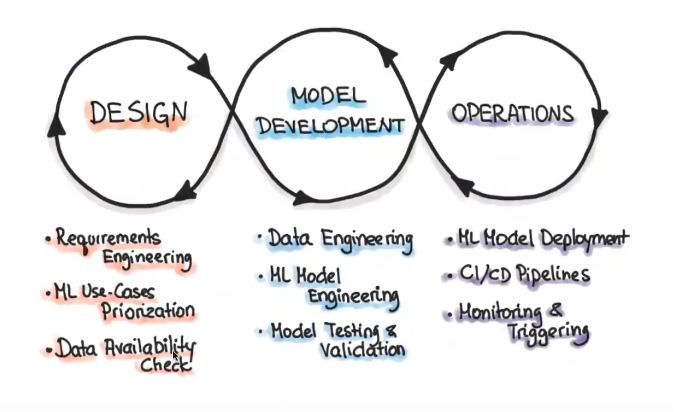
\includegraphics[scale=0.5]{proceso-mlops.png}
    \caption{Metodología MLOps}
    \label{fig:proces-mlops}
\end{figure}

Para visualizar de forma más clara la ventaja que supone este enfoque frente a uno tradicional, a continuación
se mencionara un ejemplos de una posible situacion real. \textbf{Ejemplo:} Tenemos un modelo que actualmente está alojado en AWS y queremos migrarlo a Azure, debido a que
utilizamos MLOps existe configurada una action que en el momento que el equipo publica una nueva release
automáticamente despliega el modelo en el servidor cloud. La parte del equipo encargada de las operaciones procede
a configurar el nuevo servicio y modificar la action para redirigir el despliegue al nuevo servidor. Durante este
tiempo, el equipo de desarrollo a podido avanzar en nuevas mejoras para el modelo y ahora se disponen a volver
a publicar los cambios. Ellos no han notado ningún cambio, pero a nivel de infraestructura se ha realizado una
completa migracion sin afectar en ningún momento en el desarrollo.


\pagebreak
\subsection{Metodología de investigación}
En esta sección, se describirá la metodología desarrollada para abordar problemas 
dentro del marco de trabajo de los problema NP-Hard. La metodología propuesta se 
basa en el uso de técnicas de Imitation Learning para abordar problemas computacionalmente
complejos, dando resultados cercanos al optimo en un tiempo de ejecución muy reducido. 
Se explicará cómo esta metodología se ha diseñado y aplicado para resolver el caso concreto 
del FJSP, pero como se ha mencionado anteriormente, esta metodología es aplicable a cualquier
problema NP-Hard.\medskip

Una vez que sea descrita la metodología para abordar el problema utilizando 
técnicas de Imitation Learning, se procederá con el caso especifico de cómo esta metodología 
ha sido aplicada para diseñar un modelo del FJSP. Se explicará cómo se ha procedido en cada uno 
de los pasos propuestos a nivel de razonamiento y ejecución. A continuación se van a listar una 
serie de puntos que se deben seguir para poder aplicar la metodología propuesta:

\begin{enumerate}
    \item \textbf{Modelado del problema como un environment de RL.} El problema 
    se modeliza como un environment de Reinforcement Learning, definiendo el espacio de estados 
    y el espacio de acciones disponibles para el agente. A diferencia de un enfoque típico de RL, 
    no es necesario definir una función de recompensa ya que el modelo se entrenará mediante aprendizaje 
    supervisado y no por refuerzo. Es importante destacar que el espacio de estados y el espacio de
    acciones estén enfocados en construir gradualmente la solución del problema y ser capaces
    de representar una solución valida.
    \item \textbf{Generación de instancias aleatorias para el entrenamiento del modelo.} 
    Se generan instancias aleatorias del problema con el fin de crear un conjuntos de datos 
    para el modelo de aprendizaje automático. Estas instancias aleatorias se utilizaran para entrenar el 
    modelo de deep learning, que servirá para predecir soluciones en instancias del problema no vistas 
    previamente. Una recomendación es que adicionalmente se generen diferentes grupos de instancias,
    con diferentes tamaños y características, para poder evaluar el rendimiento del modelo en diferentes
    escenarios.
    \item \textbf{Utilización de métodos de programación matemática para obtener la solución óptima de 
    las instancias.} Mediante métodos de programación matemática, se busca obtener las soluciones óptimas 
    para las instancias generadas en el paso anterior. Estas soluciones óptimas se utilizaran como los 
    datos del experto, lo que permitirá al modelo desarrollar una estrategia para resolver instancias no vistas.
    \item \textbf{Entrenamiento del modelo supervisado de deep learning.} Una vez que se tienen las instancias
    generadas y las soluciones óptimas, se procesarán a traves del environment de tal forma que para cada
    instancia se obtenga una secuencia de acciones que representan la solución óptima. Estas secuencias de
    acciones serán las que el modelo de deep learning tratará de predecir.
    \item \textbf{Evaluación de resultados y benchmark.} Se utilizó el modelo entrenado 
    en el paso anterior para predecir soluciones en instancias del problema que forman parte del benchmark 
    o conjunto de datos de prueba. El objetivo es evaluar la capacidad del modelo para generalizar y 
    proporcionar soluciones adecuadas en instancias no vistas previamente.
\end{enumerate}


\pagebreak